\documentclass[tikz,border=2mm]{standalone}
\usepackage{xcolor}
\usepackage{amsmath}
\usetikzlibrary{positioning, shapes, arrows.meta, fit, calc}

\begin{document}

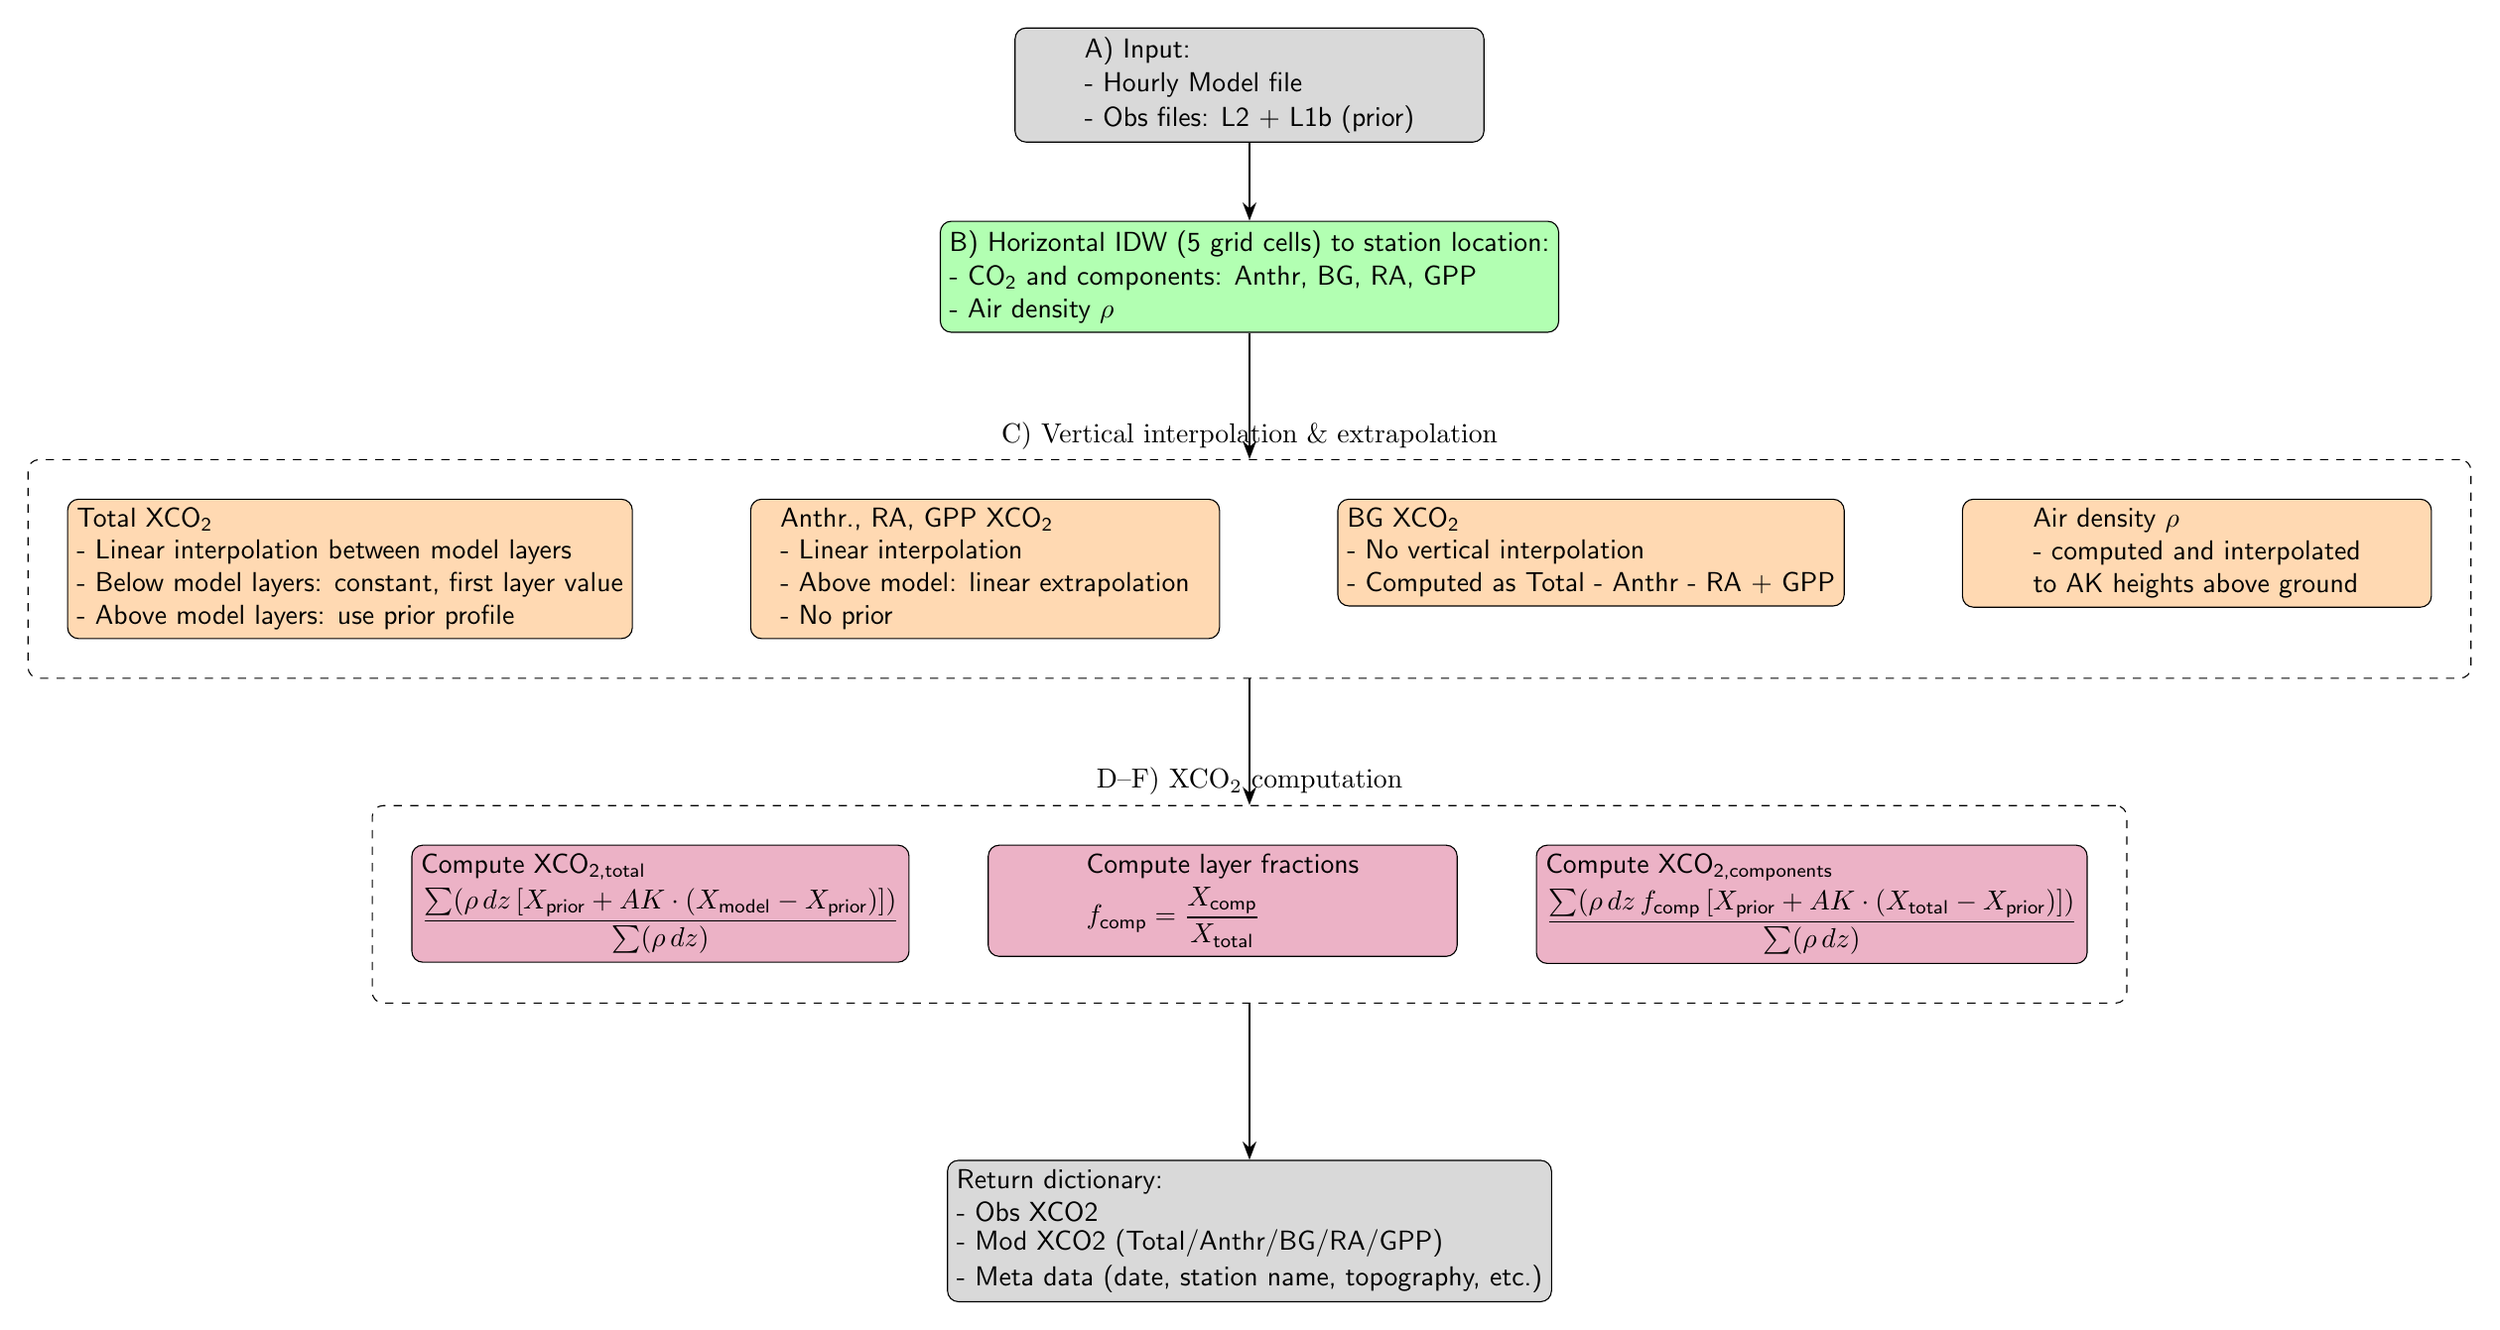
\begin{tikzpicture}[
  step/.style={rectangle, draw, rounded corners, minimum width=6cm, minimum height=1cm, text centered, font=\sffamily, fill=#1!30},
  arrow/.style={-{Stealth}, thick},
  cluster/.style={draw,dashed, rounded corners, inner sep=5mm, align=center, font=\sffamily},
  node distance=1cm
]

% ---------- Top workflow ----------
\node[step=gray] (A) {\shortstack[l]{A) Input:\\- Hourly Model file \\- Obs files: L2 + L1b (prior)}}; 
\node[step=green, below=of A] (B) {\shortstack[l]{B) Horizontal IDW (5 grid cells) to station location:\\- CO\textsubscript{2} and components: Anthr, BG, RA, GPP\\- Air density $\rho$}}; 

% ---------- Vertical Interpolation Cluster (C) ----------
\matrix[column sep=1.5cm, row sep=0cm, below=2cm of B] (Cmatrix) {
  \node[step=orange] (C1) {\shortstack[l]{Total XCO\textsubscript{2}\\- Linear interpolation between model layers\\- Below model layers: constant, first layer value\\- Above model layers: use prior profile}}; &
  \node[step=orange] (C2) {\shortstack[l]{Anthr., RA, GPP XCO\textsubscript{2}\\- Linear interpolation\\- Above model: linear extrapolation\\- No prior}}; &
  \node[step=orange] (C3) {\shortstack[l]{BG XCO\textsubscript{2}\\- No vertical interpolation\\- Computed as Total - Anthr - RA + GPP}}; & 
  \node[step=orange] (C4) {\shortstack[l]{Air density $\rho$\\- computed and interpolated\\to AK heights above ground}}; \\
};

\node[cluster, fit=(C1) (C2) (C3) (C4), label=above:C) Vertical interpolation \& extrapolation] (Ccluster) {};

% ---------- XCO2 computation cluster (D-F) ----------
\matrix[column sep=1cm, below=2cm of Ccluster] (Xmatrix) {
  \node[step=purple] (D) {\shortstack[l]{Compute XCO\textsubscript{2,total}\\$\displaystyle \frac{\sum (\rho \, dz \,[X_\text{prior} + AK \cdot (X_\text{model}-X_\text{prior})])}{\sum (\rho \, dz)}$}}; &
  \node[step=purple] (E) {\shortstack[l]{Compute layer fractions\\$\displaystyle f_\text{comp} = \frac{X_\text{comp}}{X_\text{total}}$}}; &
  \node[step=purple] (F) {\shortstack[l]{Compute XCO\textsubscript{2,components}\\$\displaystyle \frac{\sum (\rho \, dz \, f_\text{comp} \,[X_\text{prior} + AK \cdot (X_\text{total}-X_\text{prior})])}{\sum (\rho \, dz)}$}}; \\
};

\node[cluster, fit=(D) (E) (F), label=above:D--F) XCO\textsubscript{2} computation] (Xcluster) {};

% ---------- Output node ----------
\node[step=gray, below=2cm of Xcluster] (G) {\shortstack[l]{Return dictionary:\\- Obs XCO2\\- Mod XCO2 (Total/Anthr/BG/RA/GPP)\\- Meta data (date, station name, topography, etc.)}}; 

% ---------- Arrows ----------
\draw[arrow] (A) -- (B);
\draw[arrow] (B.south) -- (Ccluster.north);
\draw[arrow] (Ccluster.south) -- (Xcluster.north);
\draw[arrow] (Xcluster.south) -- (G.north);

\end{tikzpicture}

\end{document}
